
\chapter{Einfluss der Auger-Rekombination auf die IQE}
\label{chap:auger}
\thispagestyle{fancy}
Das zu Beginn dieser Arbeit verwendete Modell zur Bestimmung der PL-IQE ging davon aus, dass bei Tieftemperatur keine Auger-Rekombination (Gleichung \ref{eq:standardiqe}) vorkommt. Wie in Abb. \ref{fig:auger5k} deutlich zu erkennen ist, nimmt jedoch die Steigung der PL-Intensität in doppeltlogarithmischer Darstellung in Abhängigkeit der Anregungsleistungsdichte im Bereich höherer Anregungsleistungen deutlich ab. Die PL-Intensität weist dann keinen linearen Verlauf mehr auf, den sie aber durch eine allein quadratische Abhängigkeit (in doppeltlogarithmischer Darstellung linear) haben sollte. 
\newline
\begin{figure}[ht]
    \centering
    \begin{minipage}[t]{0.49\linewidth}
        \centering
        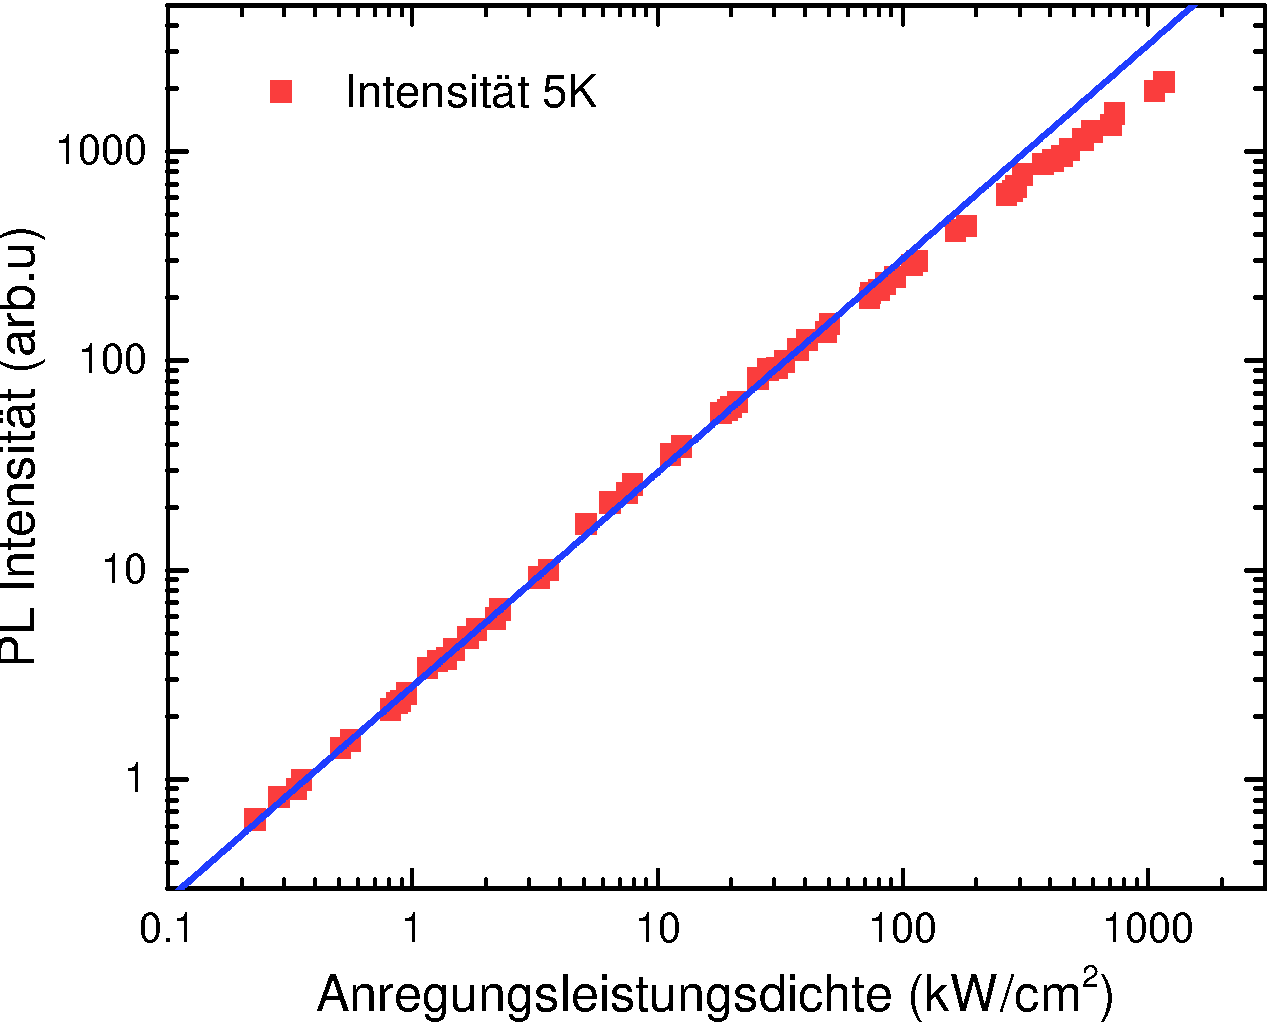
\includegraphics[width=\linewidth]{Bilder/AugerBei5K.pdf}
        \caption{Die Grafik zeigt die integrierte Intensität bei Tieftemperatur ($5 K$) in Abhängigkeit der Anregungsleistungdichte. In doppeltlogarithmischer Darstellung müsste die integrierte Intensität wegen $R = B \cdot n^2$ linear steigen (schwarze Linie).}
        \label{fig:auger5k}
    \end{minipage}% <- sonst wird hier ein Leerzeichen eingefügt
    \hfill
    \begin{minipage}[t]{0.49\linewidth}
        \centering
        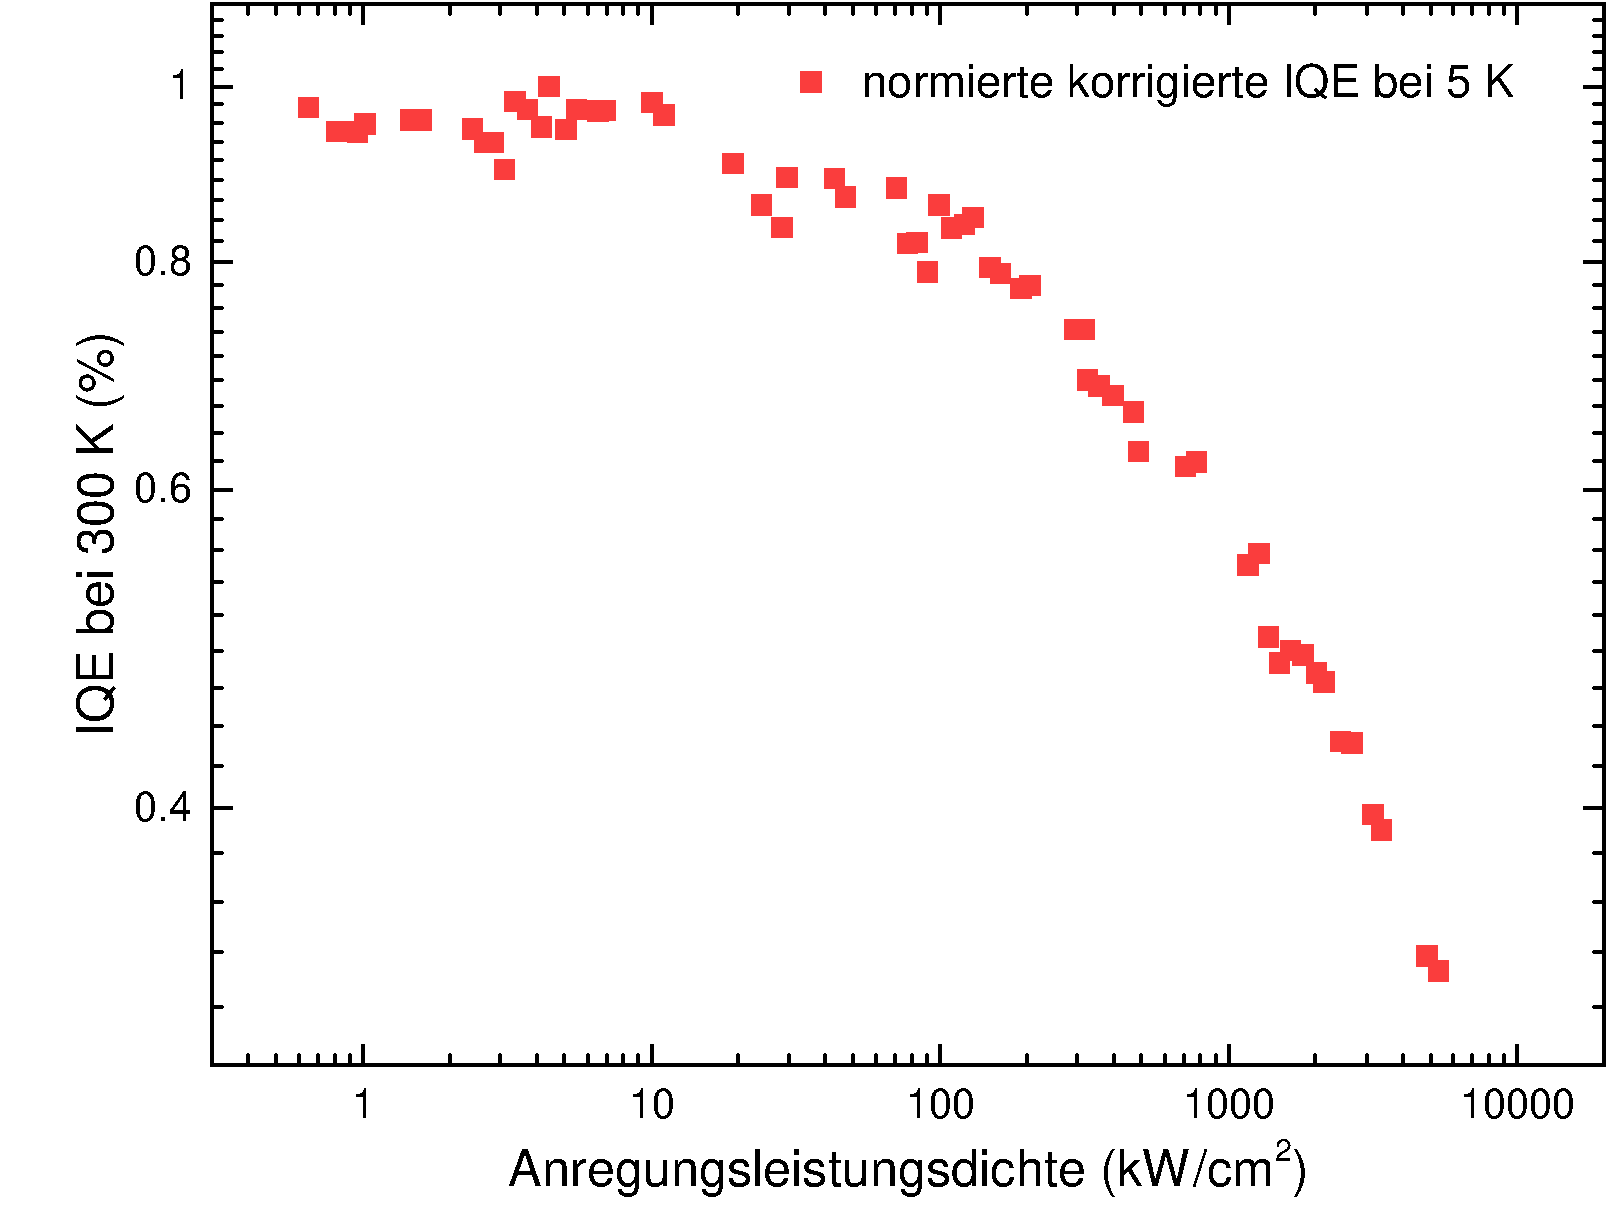
\includegraphics[width=\linewidth]{Bilder/NormierteKorrgierteIQE5K.pdf}
        \caption{Die Grafik zeigt die normierte korrigierte IQE bei 5K nach Gleichung \ref{eq:iqetrue5k}}
        \label{fig:trueiqe}
    \end{minipage}
\end{figure}
\vspace{0.1cm}
\noindent
\newline
Dies zeigt, dass die IQE bei Tieftemperatur entgegen der bisherigen Annahme, nicht immer bei 100 Prozent liegt, sondern auch von der  Anregungsleistungsdichte abhängig ist. Dass dieser Verlustmechanismus ähnlich wie bei InGaN/GaN auf Auger-Rekombination, wurde von Nippert et al. bestätigt \cite{doi:10.1063/1.4965298}. 
\newline
Um dies zu berücksichtigen, wird nun die IQE bei 5K definiert als:
\begin{equation}
    IQE_{corr}(T = 5K, P_{exc}) = \frac{ \frac{I_{pl}(T,P_{exc}) }{P_{exc} } } { I_{norm}}
    \label{eq:iqetrue5k}
\end{equation}
mit dem Maximum der Verhältnisse von integrierter PL-Intensität zu Anregungsleistungdichte als  Normierungsfaktor über alle $n$ Anregungsleistungdichten:
\begin{equation}
    I_{norm} = \lvert \lvert \sum_{i=1}^{n} \frac{I_{pl}(T,P_{exc,i})}{P_{exc,i}} \lvert \lvert_{max}
    \label{eq:iplnorm}
\end{equation}
\noindent
\begin{figure}[htb]
\centering
    \begin{minipage}[t]{0.49\linewidth}
        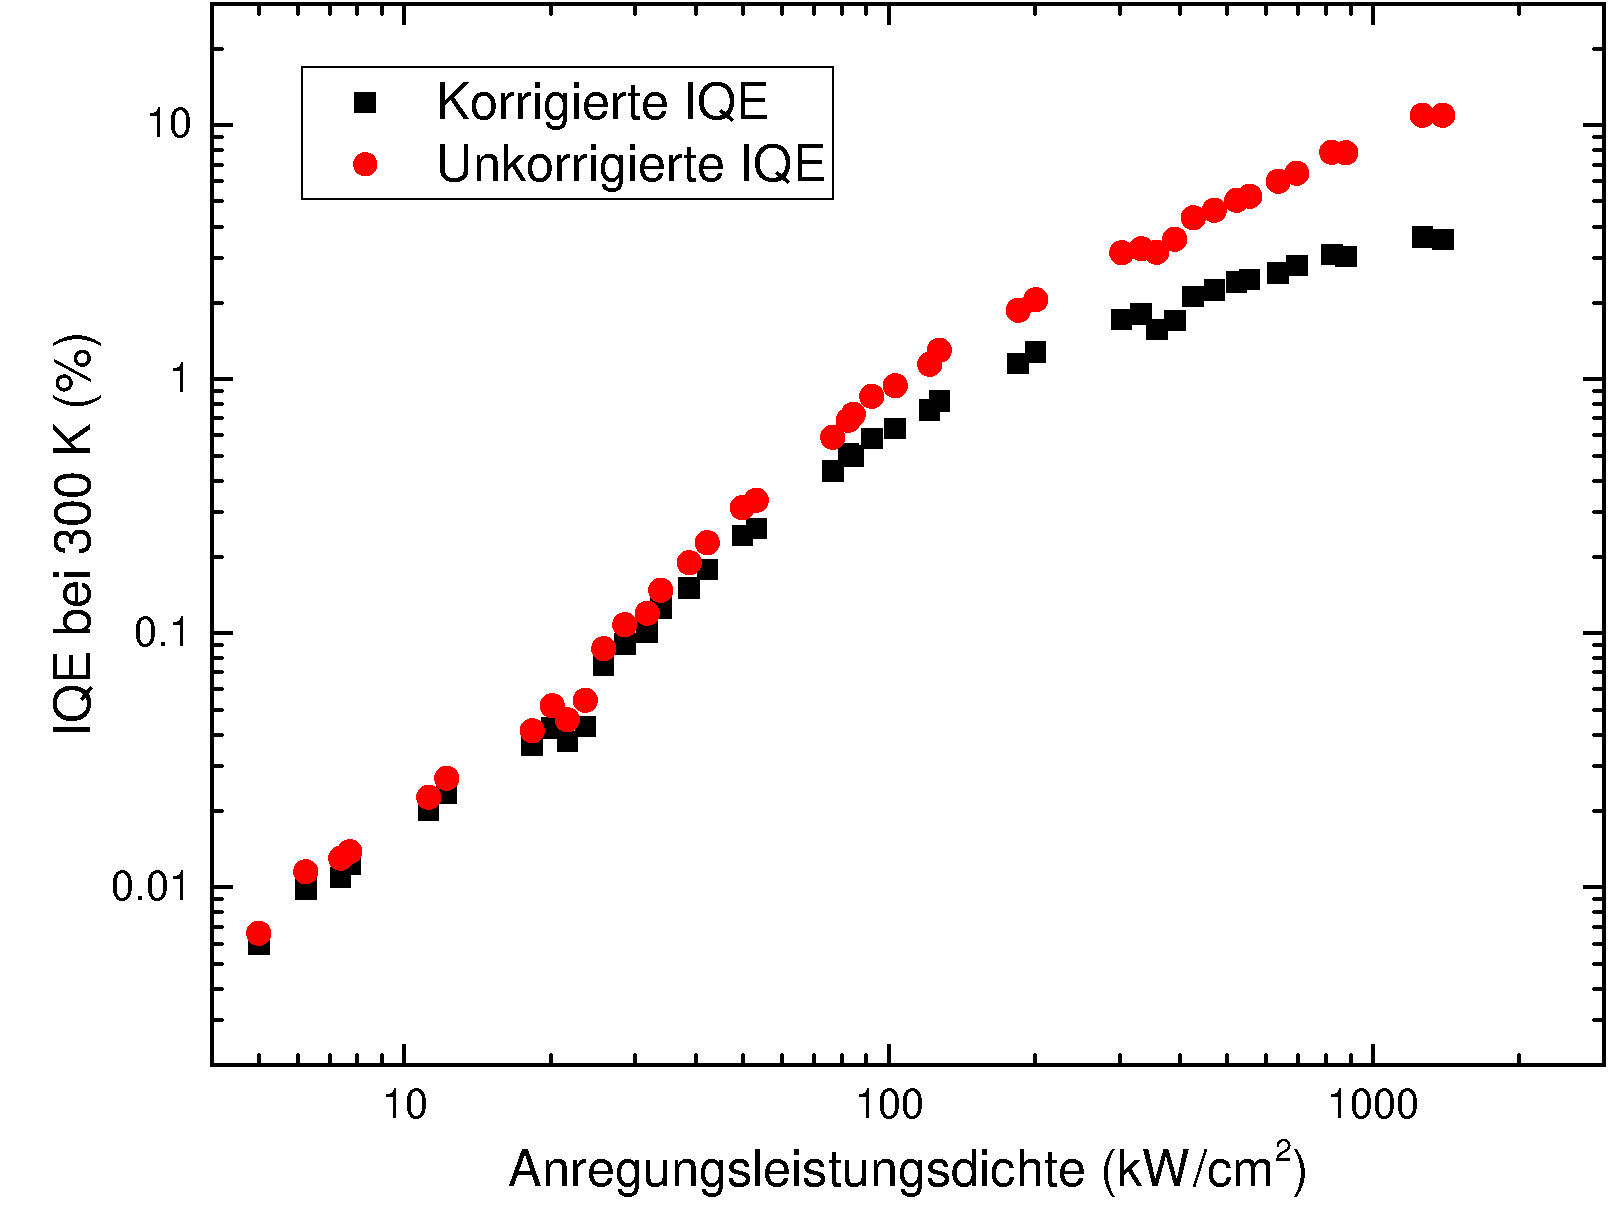
\includegraphics[width=\linewidth]{Bilder/korrigierteIQE300K.pdf}
        \caption{Vergleich von korrigierter und unkorrigierter IQE bei 300K nach Gleichung \ref{eq:iqetrue300k} }
        \label{fig:trueiqe300k}
    \end{minipage}
\end{figure}
\noindent
\newline
So ist $I_{pl}(P_{exc})$ die von der Anregungsleistungsdichte $P_{exc}$ und Temperatur $T = 5K$ abhängige integrierte PL-Intensität. Die integrierte PL-Intensität wird durch die Anregungsleistungsdichte dividiert und auf das Maximum normiert, so dass die höchste IQE bei Tieftemperatur im Bereich der geringsten Anregungsleistungdichte mit der geringsten Auger-Rekombination liegen sollte. Um nun die IQE bei Raumtemperatur zu bestimmen, wird die nach dem alten Verfahren ermittelte IQE mit den neu ermittelten Werten passend zur Anregungsleistungsdichte multipliziert (Abb. \ref{fig:trueiqe300k}). 
\begin{equation}
    IQE_{corr}(T, A_{exc}) = \frac{IQE(T,A_{exc})}{IQE(5K,A_{exc})} \cdot IQE_{corr}(5K,A_{exc})
    \label{eq:iqetrue300k}
\end{equation}
Die IQE bei $5K$ dient hierbei also als Skalierungsfaktor, der den Einfluss der Auger-Rekombination bei einer bestimmten höher liegenden Temperatur (bspw. Raumtemperatur) korrigiert. Somit fällt im Vergleich insbesondere auf, dass die Skalierung bei den kleinsten Anregungsleistungsdichten den geringsten Einfluss hat und mit steigender Anregungsleistungsdichte kubisch steigt. Daher müssen die nach dem alten Verfahren ermittelten IQE-Werte bei höheren Anregungsleistungsdichten deutlich nach unten korrigiert werden. \newline
Auch wenn mit diesem Verfahren der Einfluss der Auger-Rekombination berücksichtigt wird, gibt es noch weitere Einflüsse die bei der IQE-Bestimmung beachtet werden müssen. Ein erhebliches Problem steckt in der nicht-resonanten Anregung mit dem ArF-Excimer Laser. Das Laserlicht wird wegen der hohen Energie von allen Schichten und damit insbesondere in den Barrieren absorbiert. Die angeregten Ladungsträger müssen in den QW diffundieren und dort relaxieren, rekombinieren aber potentiell in den Barrieren, was im Spektrum als Barrieren Peak speziell bei Tieftemperatur zu sehen ist.
\newline
Daraus und aus Absorption resultierend, scheitern AlGaN-Heterostrukturen, die mit einem ArF Laser angeregt werden, oft dabei eine Sättigung in der IQE zu erreichen \cite{doi:10.1063/1.4965298}. Ohne Sättigung ist es schwierig eine echte IQE anzugeben, da die in QWs gelangende Laserstrahlung, von nicht-resonanter Anregung ausgehend, von Materialparametern wie Absorptionskoeffizient und thermischer Diffusion abhängen. Somit ist nicht klar, welche Anregungsleistungsdichte tatsächlich in die QWs gelangt. Deswegen ist ein Vergleich von Proben, die sich in ihren Absorptionseigenschaften stark unterscheiden, schwer zu vergleichen, wenn die maximale IQE nicht bestimmt werden kann \cite{doi:10.1063/1.5044383}. 

